\documentclass[a4paper, 12pt]{article} 
\usepackage{tikz} 
  \usepackage{tikz,fullpage} 
  \usetikzlibrary{arrows,% 
  	petri,% 
  	topaths}% 
  \usepackage{tkz-berge} 
  \usepackage[position=top]{subfig} 
  \usepackage{amsmath} 
  \usepackage{amsfonts} 
  \usepackage{amssymb} 
  \usepackage{graphicx} 
  \usepackage{textcomp} 
  \usepackage{logicproof} 
  \usepackage{float} 

\begin{document} 
\title{Mathematics for Computer Science Summative Assignment 2018-19} 
\author{clvp22} %REPLACE WITH YOUR CIS CODE 

\maketitle 

 
  
 
\section{Discrete Mathematics and Linear Algebra} 
\subsection{} 
Inductive proof, so mostly text. Text is just written as normal, if you want to include maths notation in line you use the $\$$ symbol we $n\geq 1$. 
If you use $\$\$$ it will go on a separate line. $$2(\sqrt{n+1}-1)<1 + \frac{1}{\sqrt{2}} + ... + \frac{1}{\sqrt{n}} < 2\sqrt{n}$$ 
\subsection{} 
You might want some Greek letters eg $\sigma$ and $\Sigma$ or maybe to square things $a^{2} = b^{2} +c^{2}$- 
\subsection{} 
Some answer for q3 
\subsection{} 
GRAPHS 
\begin{figure}[] 
	\begin{center} 
 	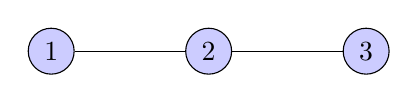
\begin{tikzpicture}[main_node/.style={circle,fill=blue!20,draw,minimum size=1em,inner sep=3pt]}] 
 	 
 	\node[main_node] (1) at (0,0) {1}; 
 	\node[main_node] (2) at (2,0) {2}; 
 	\node[main_node] (3) at (4,0) {3}; 
 	\draw (1) -- (2) -- (3); 
 
 
 	\end{tikzpicture} 
 	\end{center} 
 	\caption{$P_{3}$} 
 	\label{P3} 
\end{figure} 
\begin{figure}[H] 
 	\begin{center} 
 		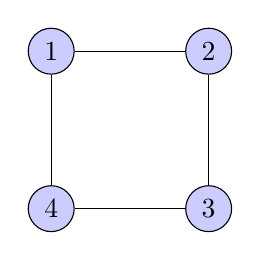
\begin{tikzpicture}[main_node/.style={circle,fill=blue!20,draw,minimum size=1em,inner sep=3pt]}] 
 		 
 		\node[main_node] (4) at (0,0) {4}; 
 		\node[main_node] (3) at (2,0) {3}; 
 		\node[main_node] (2) at (2,2) {2}; 
 		\node[main_node] (1) at (0,2) {1}; 
 		\draw (1) -- (2) -- (3) -- (4) -- (1); 
 		 
 		\end{tikzpicture} 
 	\end{center} 
 	\caption{$C_{4}$} 
 	\label{C4} 
\end{figure} 
\begin{figure}[H] 
 	\begin{center} 
 		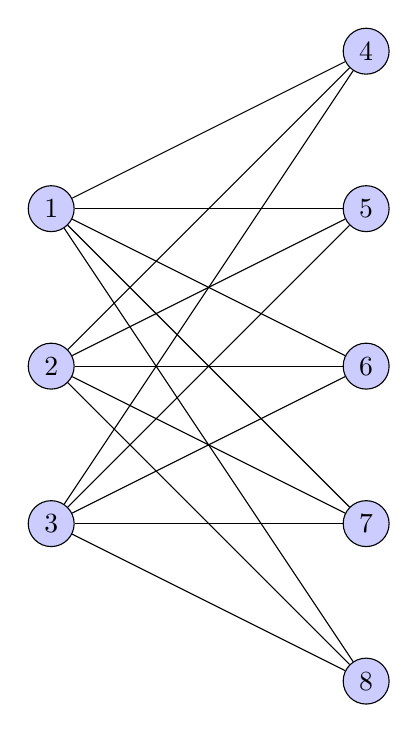
\begin{tikzpicture}[main_node/.style={circle,fill=blue!20,draw,minimum size=1em,inner sep=3pt]}] 
 		 
 		\node[main_node] (3) at (0,2) {3}; 
 		\node[main_node] (2) at (0,4) {2}; 
 		\node[main_node] (1) at (0,6) {1}; 
 		\node[main_node] (8) at (4,0) {8}; 
 		\node[main_node] (7) at (4,2) {7}; 
 		\node[main_node] (6) at (4,4) {6}; 
 		\node[main_node] (5) at (4,6) {5}; 
 		\node[main_node] (4) at (4,8) {4}; 
  		 
  		\draw (1) -- (4); 
 		\draw (2) -- (4); 
  		\draw (3) -- (4); 
  		\draw (1) -- (5); 
  		\draw (2) -- (5); 
  		\draw (3) -- (5); 
  		\draw (1) -- (6); 
  		\draw (2) -- (6); 
  		\draw (3) -- (6); 
  		\draw (1) -- (7); 
  		\draw (2) -- (7); 
  		\draw (3) -- (7); 
  		\draw (1) -- (8); 
  		\draw (2) -- (8); 
  		\draw (3) -- (8); 
  		\end{tikzpicture} 
 	\end{center} 
  	\caption{$K_{3,5}$} 
  	\label{K3,5} 
\end{figure} 
The graph in figure\ref{P3} is $P_{3}$, i.e. a path on 3 nodes. 
\\ 
The graph in figure\ref{C4} is $C_{4}$. i.e. a cycle on 4 nodes. 
\\ 
The graph in figure\ref{K3,5} is $K_{3,5}$, i.e. the complete bipartite graph with sets of size 3 and 5. 
\newpage 
\section{Logic and Discrete Structures} 
\subsection{} 
$\varphi = ((a \wedge b)\implies c) \wedge(a \vee b)$ 
\subsubsection{} 
\begin{tabular}{|c|c|c|c|c|} 
 	\hline  
  	&  &  &  &  \\  
  	\hline  
 	&  &  &  &  \\  
 	\hline  
  	&  &  &  &  \\  
  	\hline  
  	&  &  &  &  \\  
  	\hline  
  	&  &  &  &  \\  
  	\hline  
  	&  &  &  &  \\  
  	\hline  
  	&  &  &  &  \\  
  	\hline  
\end{tabular}  
\subsubsection{} 
Since I've not used it yet: $\neg \varphi$ 
\subsection{} 
$\{\wedge,\oplus\} $ where $p\oplus q \equiv\neg (p\iff q)$ 
\subsection{} 
$p \vee (q \wedge r) \vdash p \vee q$  
\\ 
\begin{logicproof}{2} 
  	p \lor (q \land r) & Premise 
  	\\ 
  	\begin{subproof} 
  		p & Assumption 
  		\\ 
 		p \lor q & \lor_{i}, 2 
  	\end{subproof} 
  	\begin{subproof} 
  		q \land r & Assumption 
  		\\ 
  		q & \land_{e}, 4 
 		\\ 
  		p \lor q & \lor_{i}, 5 
 	\end{subproof} 
  	p \lor q & \lor_{e}, 1, 2--3, 4--6 
\end{logicproof} 
\subsection{} 
I guess y'all need another subsection anyway 
\end{document} 
